\documentclass[11pt,a4paper,twocolumn]{article}
\usepackage[utf8]{inputenc}
\usepackage{amsmath}
\usepackage{graphicx}
\usepackage{hyperref}
\usepackage{setspace}
\usepackage{enumerate}
\usepackage[inline]{enumitem}   
\title{Assignment10}
\author{Aravind A Anil}
\date{\today}
\begin{document}
\maketitle

\textbf{Problem Statement:}Two independent random variables X and Y
are uniformly distributed in the interval [-1,1].The probability that max [X,Y] is less than $\frac{1}{2}$ is\\[5pt]
\begin{enumerate*}[label=\alph*)]
    \item $\frac{3}{4}$\hspace{.5cm}
    \item $\frac{9}{16}$\hspace{.5cm}
    \item $\frac{1}{4}$\hspace{.5cm}
    \item $\frac{2}{3}$\hspace{.5cm}
\end{enumerate*}\\[5pt]
X and Y are having uniform distribution\\
\begin{equation*}
  f_{X}(x)=
\begin{cases}
\frac{1}{2} & \text{if} -1<X<1\\
0 & \text{otherwise}
\end{cases}
\end{equation*}
\begin{equation*}
     f_{Y}(y)=
     \begin{cases}
     \frac{1}{2} & \text{if} -1<Y<1\\
     0 & \text{otherwise}
     \end{cases}
\end{equation*}
$Pr(\text{max(X,Y)}<\frac{1}{2}$ implies that\\[5pt]
$X<\frac{1}{2}$ \& $Y<\frac{1}{2}$\\
Since X and Y are independent
\begin{align*}
    Pr(X<\frac{1}{2},&Y<\frac{1}{2})\\
    &=\int_{-1}^{\frac{1}{2}}\int_{-1}^{\frac{1}{2}}\frac{1}{2}.\frac{1}{2}dxdy\\
    &=\frac{1}{4}\int_{-1}^{\frac{1}{2}}\Big[\frac{1}{2}+1\Big]dy\\
    &=\frac{1}{4}.\frac{3}{2}\Big[\frac{1}{2}+1\Big]\\
    &=\frac{1}{4}\times\frac{3}{2}\times\frac{3}{2}\\
    &=\frac{9}{16}
\end{align*}
\begin{figure}
    \centering
    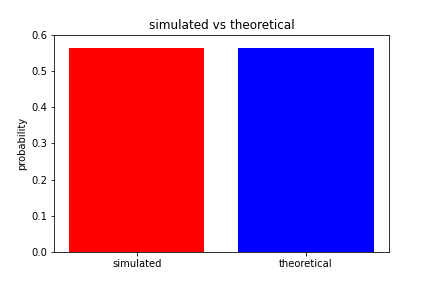
\includegraphics[width=9cm]{simulated vs theoretical.png}
    \caption{simulated vs theoretical}
    \label{fig:my_label}
\end{figure}
\end{document}
